\newpage

\section{Расчёт риск метрик}
\label{section:risk-measures}

В данном разделе приведёны результаты расчётов VaR и CVaR с использованием выбранных моделей копула. Далее проведена бутстрап-процедура с целью получения несмещённой оценки риск метрик. В последней главе получены кривые VaR и CVaR в реальном времени, проведён тест Купича.

\subsection{Упрощённый расчёт VaR и CVaR}

На данном этапе имеются массив лог-доходностей с известными для каждой переменной маргинальными распределениями, весовые коэффициенты CVaR-оптимального портфеля, три модели копула с известными параметрами. 
Для заданного в главе~\ref{calibration:optim} вектора уровней вероятностей $\pmb{\upalpha}$ вычисляем значения $\emph{VaR}_\alpha$ и $\emph{CVaR}_\alpha$ согласно алгоритму~\ref{Alg1}.

\begin{table}[bth]
\centering
\caption{VaR эмпирический и оценённый с помощью Гауссовой\,/\,Стьюдента\,/\,R-vine копул}
\label{tab:var}
\setlength{\tabcolsep}{5pt}
\begin{adjustbox}{max width=\textwidth}
\begin{tabularx}{\textwidth}{
>{\setlength{\hsize}{\hsize}}Y|
>{\setlength{\hsize}{\hsize}}Y
*{2}{|>{\setlength{\hsize}{0.4\hsize}}R
*{2}{@{\,/\,}>{\setlength{\hsize}{0.4\hsize}}R}}}
\hline
\multicolumn{1}{c|}{Уровень, \%} & \multicolumn{1}{c|}{$\widehat{\emph{VaR}}$, $\times 10^{-2}$} & \multicolumn{3}{c|}{$\emph{VaR}^{est}$, $\times 10^{-2}$} & \multicolumn{3}{c}{$\Delta$, $\times 10^{-3}$} \bigstrut[t] \\ \hline 
90   & $1.31$ & $1.57$ & $1.71$ & $1.51$ & $2.55$ & $3.94$ & $1.94$ \\ 
95   & $1.69$ & $2.15$ & $2.37$ & $1.94$ & $4.56$ & $6.81$ & $2.48$ \\ 
99   & $2.59$ & $3.28$ & $3.64$ & $3.28$ & $6.95$ & $10.54$ & $6.97$ \\ 
99.5 & $3.63$ & $3.70$ & $4.02$ & $3.94$ & $0.69$ & $3.95$ & $3.13$ \\ 
99.9 & $5.62$ & $5.63$ & $5.83$ & $6.01$ & $0.12$ & $2.18$ & $3.90$ \\ \hline
\end{tabularx}
\end{adjustbox}
\end{table}

\begin{table}[bth]
\centering
\caption{CVaR эмпирический и оценённый с помощью Гауссовой\,/\,Стьюдента\,/\,R-vine копул}
\label{tab:es}
\setlength{\tabcolsep}{5pt}
\begin{adjustbox}{max width=\textwidth}
\begin{tabularx}{\textwidth}{
>{\setlength{\hsize}{\hsize}}Y|
>{\setlength{\hsize}{\hsize}}Y
*{2}{|>{\setlength{\hsize}{0.4\hsize}}R
*{2}{@{\,/\,}>{\setlength{\hsize}{0.4\hsize}}R}}}
\hline 
\multicolumn{1}{c|}{Уровень, \%} & \multicolumn{1}{c|}{$\widehat{\emph{CVaR}}$, $\times 10^{-2}$} & \multicolumn{3}{c|}{$\emph{CVaR}^{est}$, $\times 10^{-2}$} & \multicolumn{3}{c}{$\Delta$, $\times 10^{-3}$} \bigstrut[t] \\ \hline 
90   & $2.01$ & $2.38$ & $2.58$ & $2.32$ & $3.68$ & $5.66$ & $3.12$ \\ 
95   & $2.48$ & $2.95$ & $3.17$ & $2.92$ & $4.65$ & $6.89$ & $4.35$ \\ 
99   & $3.96$ & $4.25$ & $4.35$ & $4.50$ & $2.98$ & $3.94$ & $5.41$ \\ 
99.5 & $5.22$ & $5.05$ & $4.95$ & $5.43$ & $-1.76$ & $-2.72$ & $2.06$ \\ 
99.9 & $5.86$ & $5.81$ & $6.00$ & $6.01$ & $-0.51$ & $1.38$ & $1.51$ \\ \hline
\end{tabularx}
\end{adjustbox}
\end{table}

\imgh[tbh!]{VaR-ES.pdf}{width=\textwidth}{Результаты оценки риск метрик}{smplfied-rm}

В табл.~\ref{tab:var} и \ref{tab:es} приведены результаты упрощённого расчёта VaR и CVaR.
На рис.~\ref{ris:smplfied-rm} изображены графики риск метрик: VaR (слева) и CVaR (справа). 
Насколько можно судить из таблиц и рисунка, все три модели остаются консервативными на небольших и средних уровнях вероятности. 
Причём оценки, полученные с помощью Гауссовой и Стьюдента копул, консервативнее по сравнению с более точной моделью R-вайн копулы.
Далее, на уровнях $99.5$ и $99.9\%$ модели Гауссовой и Стьюдента копул начинают вести себя агрессивно (недооценивают риск), в то время как R-вайн остаётся консервативной.
На данном этапе можно сделать выбор в пользу R-вайн копулы, затем копулы Стьюдента и в последнюю очередь Гауссовой как наименее консервативной.
Однако нам необходимо получить оценку, которую с большей уверенностью можно считать несмещённой.

\subsection{Результаты бутстрап-процедуры}

Обоснование использование бутстрап-процедуры описано в гл.~\ref{methodology:bootstrap}.
Для расчётов используется алгоритм~\ref{Alg2}.
Результат для $N=200$ процедур приведены в таблицах~\ref{tab:boot-var} и \ref{tab:boot-es} и на рис.~\ref{ris:boot-rm}.

Как видно, средние значения для всех трёх моделей очень близки друг к другу.
Вертикальные линии показывают доверительный интервал от 2.5\% до 97.5\%-ной квантили на каждом уровне.
Этот интервал увеличивается с ростом уровня риск метрики, следовательно, для вычисления меры риска на больших значениях вероятности необходимо больше наблюдений.
Величина $\Delta$ показывает смещение средних значений риск метрик от эмпирических. 
Можно заметить, что все три модели теряют свою консервативность на уровне 99.5 и 99.9\%.
Следовательно, что исследуемая модель работеает для уровней не больше 99\%, что для финансовых моделей вполне достаточно.

\begin{table}[bt]
\centering
\caption{VaR эмпирический и оценённый с помощью Гауссовой\,/\,Стьюдента\,/\,R-vine копул. Бутстрап-процедура}
\label{tab:boot-var}
\setlength{\tabcolsep}{5pt}
\begin{adjustbox}{max width=\textwidth}
\begin{tabular}{c*{4}{|r@{\,/\,}r@{\,/\,}r}} \hline
\multicolumn{1}{c|}{Уровень, \%} & \multicolumn{3}{c|}{$\overline{\emph{VaR}}_\alpha$, $\times 10^{-2}$} & \multicolumn{3}{c|}{$\Delta, \times 10^{-3}$} & \multicolumn{3}{c|}{SD, $\times 10^{-2}$} & \multicolumn{3}{c}{RMSE, $\times 10^{-3}$} \\ \hline
90   & $1.61$ & $1.62$ & $1.61$ & $2.99$ &  $3.03$ &  $2.96$ & $0.80$ & $0.79$ & $0.85$ & $3.10$ & $3.13$ & $3.08$ \\
95   & $2.19$ & $2.20$ & $2.18$ & $5.00$ &  $5.06$ &  $4.93$ & $1.18$ & $1.37$ & $1.48$ & $5.14$ & $5.24$ & $5.14$ \\
99   & $3.46$ & $3.50$ & $3.46$ & $8.71$ &  $9.11$ &  $8.78$ & $1.79$ & $2.32$ & $2.47$ & $8.89$ & $9.40$ & $9.11$ \\
99.5 & $4.04$ & $4.21$ & $4.09$ & $4.15$ &  $5.82$ &  $4.64$ & $4.22$ & $6.10$ & $5.69$ & $5.91$ & $8.42$ & $7.33$ \\
99.9 & $5.62$ & $5.53$ & $5.49$ & $0.05$ & $-0.86$ & $-1.21$ & $3.81$ & $5.18$ & $5.16$ & $3.81$ & $5.24$ & $5.29$ \\ \hline
\end{tabular}
\end{adjustbox}
\end{table}

\begin{table}[bt]
\centering
\caption{CVaR эмпирический и оценённый с помощью Гауссовой\,/\,Стьюдента\,/\,R-vine копул. Бутстрап-процедура}
\label{tab:boot-es}
\setlength{\tabcolsep}{5pt}
\begin{adjustbox}{max width=\textwidth}
\begin{tabular}{c*{4}{|r@{\,/\,}r@{\,/\,}r}} \hline
\multicolumn{1}{c|}{Уровень, \%} & \multicolumn{3}{c|}{$\overline{\emph{CVaR}}_\alpha$, $\times 10^{-2}$} & \multicolumn{3}{c|}{$\Delta, \times 10^{-3}$} & \multicolumn{3}{c|}{SD, $\times 10^{-2}$} & \multicolumn{3}{c}{RMSE, $\times 10^{-3}$} \\ \hline
90   & $2.46$ & $2.47$ & $2.45$ &  $4.53$ &  $4.62$ &  $4.43$ & $1.08$ & $1.32$ & $1.35$ & $4.66$ & $4.80$ & $4.63$ \\ 
95   & $3.06$ & $3.08$ & $3.05$ &  $5.78$ &  $5.92$ &  $5.62$ & $1.49$ & $1.90$ & $1.91$ & $5.97$ & $6.21$ & $5.93$ \\ 
99   & $4.36$ & $4.40$ & $4.34$ &  $4.08$ &  $4.46$ &  $3.86$ & $3.05$ & $4.31$ & $4.21$ & $5.09$ & $6.19$ & $5.71$ \\ 
99.5 & $5.00$ & $4.99$ & $4.94$ & $-2.26$ & $-2.31$ & $-2.86$ & $4.05$ & $5.40$ & $5.34$ & $4.63$ & $5.87$ & $6.05$ \\ 
99.9 & $5.76$ & $5.68$ & $5.68$ & $-1.03$ & $-1.79$ & $-1.88$ & $2.45$ & $3.86$ & $3.52$ & $2.65$ & $4.25$ & $3.98$ \\ \hline
\end{tabular}
\end{adjustbox}
\end{table}

\imgh[bth!]{VaR-ES-Bootstrap.pdf}{width=\textwidth}{Результаты бутстрап-процедуры}{boot-rm}

\subsection{Кривые VaR и CVaR}
\label{riskmeasures:curve}

Выбрав для тренировки модели первые три месяца, я построил кривые VaR и CVaR на уровне 95\% и проверил их тестом Купича.
В качестве <<эталонных>> я использую кривые риск метрик, полученные методом исторического моделирования, описанного уравнениями~(\ref{PnL}), (\ref{VaR-hist}) и (\ref{ES-hist}).
По результатам на рис.~\ref{ris:VaR-ES-curve} 
% и \ref{ris:ES-curve} 
видно, что все три модели копула являются консвервативными, причём модель R-вайн оценивает риск точнее остальных.

По результатам теста Купича для кривых VaR, представленным в таблице~\ref{tab:kupiec}, модель $t$ копула является неадекватной и не может быть использована для оценки риска в реальном времени.
Данные результаты согласуются с результатами GoF-тестов (табл.~\ref{tab:coptest}), в которых было получено крайнее значение $p$-value для $t$ копулы.

\begin{table}[h]
    \centering
    \caption{Теста Купича для кривых VaR на 95\%}
    \label{tab:kupiec}
    \setlength{\tabcolsep}{10pt}
    \begin{tabular}{l|c|c} \hline
        Метод & LR-статистика & $p$-value \\ \hline
        эмпирический & 0 & 0.98 \\
        Гауссова копула & 3.02 & 0.08 \\
        $t$ копула & 10.29 & 0.00 \\
        R-vine & 2.17 & 0.14 \\ \hline
    \end{tabular}
\end{table}

% \imgh[thb!]{VaRcurve.pdf}{width=\textwidth}{График P\&L и кривые VaR}{VaR-curve}
% \imgh[thb!]{EScurve.pdf}{width=\textwidth}{График P\&L и кривые CVaR}{ES-curve}

\begin{figure}[p]
    \centering
    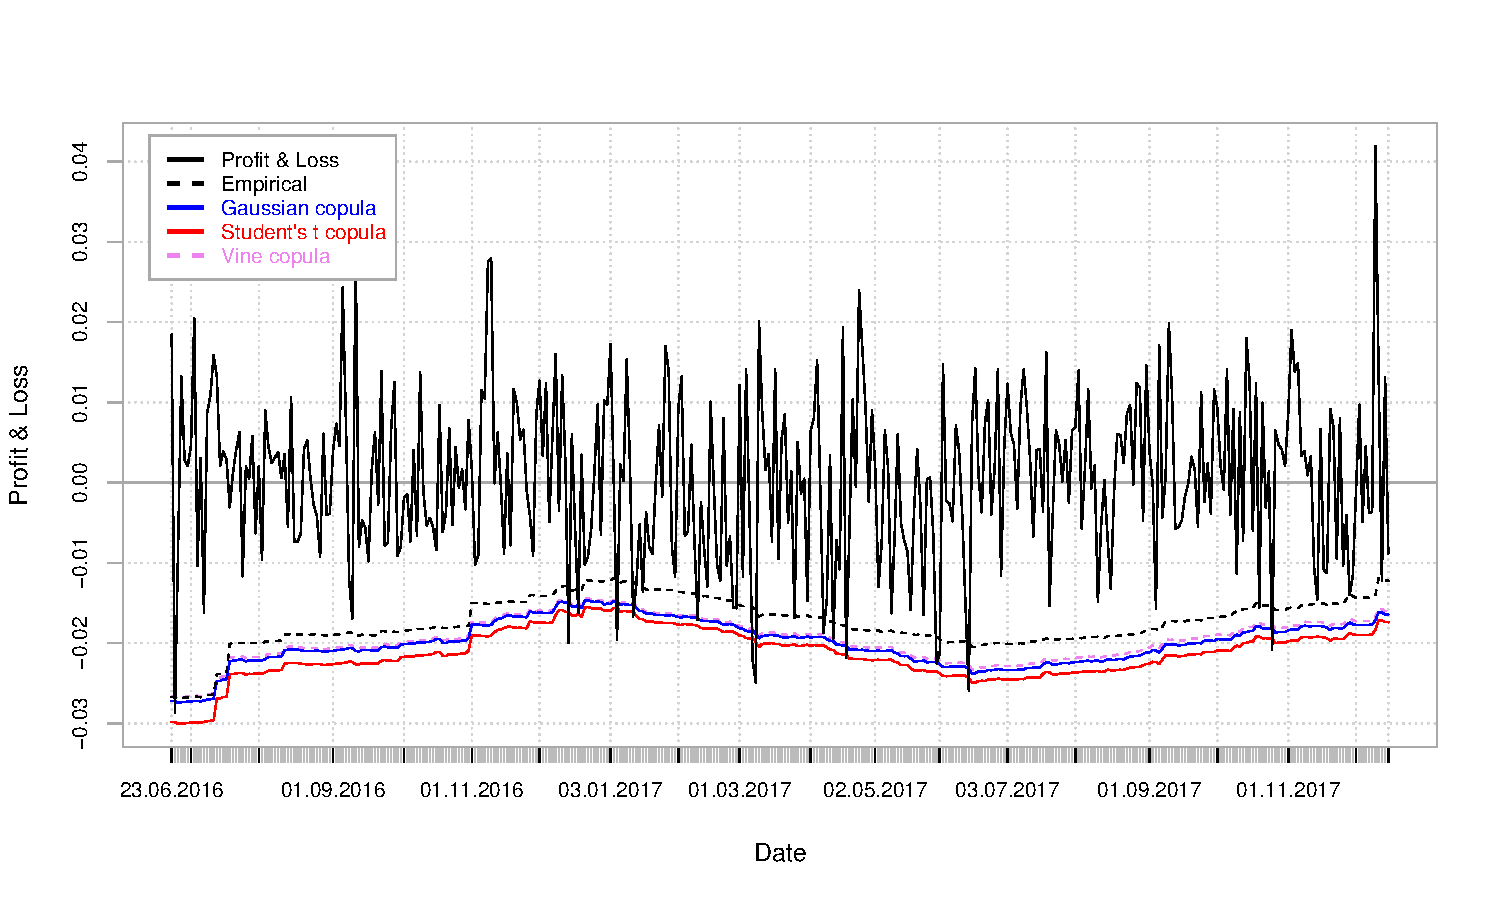
\includegraphics[width=\textwidth]{VaRcurve.pdf}
    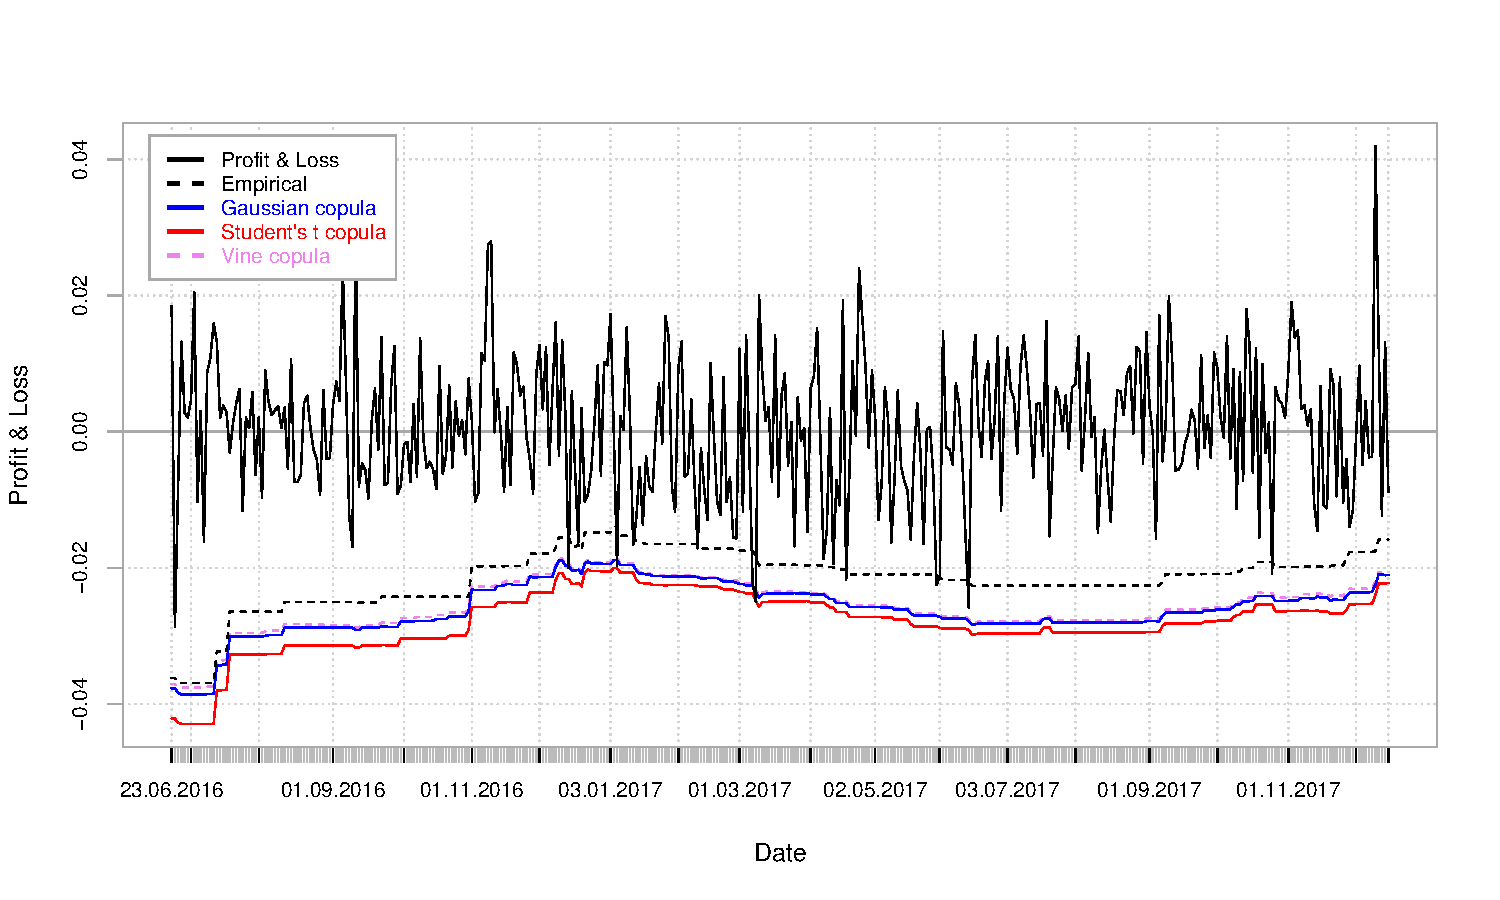
\includegraphics[width=\textwidth]{EScurve.pdf}
    \caption{Графики P\&L и кривыx VaR (сверху) и CVaR (снизу)}
    \label{ris:VaR-ES-curve}
\end{figure}